\documentclass{article}

\usepackage{hyperref}
\hypersetup{
	colorlinks=true,
	linkcolor=blue,
	urlcolor=cyan,}
\usepackage{booktabs}
\usepackage{textgreek}

%%%%%%%%%%%%%%%%%%%%%%%%%%%%%%%%%%%%%%%%%
% Lachaise Assignment
% Structure Specification File
% Version 1.0 (26/6/2018)
%
% This template originates from:
% http://www.LaTeXTemplates.com
%
% Authors:
% Marion Lachaise & François Févotte
% Vel (vel@LaTeXTemplates.com)
%
% License:
% CC BY-NC-SA 3.0 (http://creativecommons.org/licenses/by-nc-sa/3.0/)
% 
%%%%%%%%%%%%%%%%%%%%%%%%%%%%%%%%%%%%%%%%%

%----------------------------------------------------------------------------------------
%	PACKAGES AND OTHER DOCUMENT CONFIGURATIONS
%----------------------------------------------------------------------------------------

\usepackage{amsmath,amsfonts,stmaryrd,amssymb} % Math packages

\usepackage{enumerate} % Custom item numbers for enumerations

\usepackage[ruled]{algorithm2e} % Algorithms

\usepackage[framemethod=tikz]{mdframed} % Allows defining custom boxed/framed environments

\usepackage{listings} % File listings, with syntax highlighting
\lstset{
	basicstyle=\ttfamily, % Typeset listings in monospace font
}

%----------------------------------------------------------------------------------------
%	DOCUMENT MARGINS
%----------------------------------------------------------------------------------------

\usepackage{geometry} % Required for adjusting page dimensions and margins

\geometry{
	paper=a4paper, % Paper size, change to letterpaper for US letter size
	top=2.5cm, % Top margin
	bottom=3cm, % Bottom margin
	left=2.5cm, % Left margin
	right=2.5cm, % Right margin
	headheight=14pt, % Header height
	footskip=1.5cm, % Space from the bottom margin to the baseline of the footer
	headsep=1.2cm, % Space from the top margin to the baseline of the header
	%showframe, % Uncomment to show how the type block is set on the page
}

%----------------------------------------------------------------------------------------
%	FONTS
%----------------------------------------------------------------------------------------

\usepackage[utf8]{inputenc} % Required for inputting international characters
\usepackage[T1]{fontenc} % Output font encoding for international characters

\usepackage{XCharter} % Use the XCharter fonts

%----------------------------------------------------------------------------------------
%	COMMAND LINE ENVIRONMENT
%----------------------------------------------------------------------------------------

% Usage:
% \begin{commandline}
%	\begin{verbatim}
%		$ ls
%		
%		Applications	Desktop	...
%	\end{verbatim}
% \end{commandline}

\mdfdefinestyle{commandline}{
	leftmargin=10pt,
	rightmargin=10pt,
	innerleftmargin=15pt,
	middlelinecolor=black!50!white,
	middlelinewidth=2pt,
	frametitlerule=false,
	backgroundcolor=black!5!white,
	frametitle={Command Line},
	frametitlefont={\normalfont\sffamily\color{white}\hspace{-1em}},
	frametitlebackgroundcolor=black!50!white,
	nobreak,
}

% Define a custom environment for command-line snapshots
\newenvironment{commandline}{
	\medskip
	\begin{mdframed}[style=commandline]
}{
	\end{mdframed}
	\medskip
}

%----------------------------------------------------------------------------------------
%	FILE CONTENTS ENVIRONMENT
%----------------------------------------------------------------------------------------

% Usage:
% \begin{file}[optional filename, defaults to "File"]
%	File contents, for example, with a listings environment
% \end{file}

\mdfdefinestyle{file}{
	innertopmargin=1.6\baselineskip,
	innerbottommargin=0.8\baselineskip,
	topline=false, bottomline=false,
	leftline=false, rightline=false,
	leftmargin=2cm,
	rightmargin=2cm,
	singleextra={%
		\draw[fill=black!10!white](P)++(0,-1.2em)rectangle(P-|O);
		\node[anchor=north west]
		at(P-|O){\ttfamily\mdfilename};
		%
		\def\l{3em}
		\draw(O-|P)++(-\l,0)--++(\l,\l)--(P)--(P-|O)--(O)--cycle;
		\draw(O-|P)++(-\l,0)--++(0,\l)--++(\l,0);
	},
	nobreak,
}

% Define a custom environment for file contents
\newenvironment{file}[1][File]{ % Set the default filename to "File"
	\medskip
	\newcommand{\mdfilename}{#1}
	\begin{mdframed}[style=file]
}{
	\end{mdframed}
	\medskip
}

%----------------------------------------------------------------------------------------
%	NUMBERED QUESTIONS ENVIRONMENT
%----------------------------------------------------------------------------------------

% Usage:
% \begin{question}[optional title]
%	Question contents
% \end{question}

\mdfdefinestyle{question}{
	innertopmargin=1.2\baselineskip,
	innerbottommargin=0.8\baselineskip,
	roundcorner=5pt,
	nobreak,
	singleextra={%
		\draw(P-|O)node[xshift=1em,anchor=west,fill=white,draw,rounded corners=5pt]{%
		Question \theQuestion\questionTitle};
	},
}

\newcounter{Question} % Stores the current question number that gets iterated with each new question

% Define a custom environment for numbered questions
\newenvironment{question}[1][\unskip]{
	\bigskip
	\stepcounter{Question}
	\newcommand{\questionTitle}{~#1}
	\begin{mdframed}[style=question]
}{
	\end{mdframed}
	\medskip
}

%----------------------------------------------------------------------------------------
%	WARNING TEXT ENVIRONMENT
%----------------------------------------------------------------------------------------

% Usage:
% \begin{warn}[optional title, defaults to "Warning:"]
%	Contents
% \end{warn}

\mdfdefinestyle{warning}{
	topline=false, bottomline=false,
	leftline=false, rightline=false,
	nobreak,
	singleextra={%
		\draw(P-|O)++(-0.5em,0)node(tmp1){};
		\draw(P-|O)++(0.5em,0)node(tmp2){};
		\fill[black,rotate around={45:(P-|O)}](tmp1)rectangle(tmp2);
		\node at(P-|O){\color{white}\scriptsize\bf !};
		\draw[very thick](P-|O)++(0,-1em)--(O);%--(O-|P);
	}
}

% Define a custom environment for warning text
\newenvironment{warn}[1][Warning:]{ % Set the default warning to "Warning:"
	\medskip
	\begin{mdframed}[style=warning]
		\noindent{\textbf{#1}}
}{
	\end{mdframed}
}

%----------------------------------------------------------------------------------------
%	INFORMATION ENVIRONMENT
%----------------------------------------------------------------------------------------

% Usage:
% \begin{info}[optional title, defaults to "Info:"]
% 	contents
% 	\end{info}

\mdfdefinestyle{info}{%
	topline=false, bottomline=false,
	leftline=false, rightline=false,
	nobreak,
	singleextra={%
		\fill[black](P-|O)circle[radius=0.4em];
		\node at(P-|O){\color{white}\scriptsize\bf i};
		\draw[very thick](P-|O)++(0,-0.8em)--(O);%--(O-|P);
	}
}

% Define a custom environment for information
\newenvironment{info}[1][Info:]{ % Set the default title to "Info:"
	\medskip
	\begin{mdframed}[style=info]
		\noindent{\textbf{#1}}
}{
	\end{mdframed}
}
 % Include the file specifying the document structure and custom commands

%----------------------------------------------------------------------------------------
%	ASSIGNMENT INFORMATION
%----------------------------------------------------------------------------------------

\title{OIA Lab 1: In Class Assignment}
\author{BIOE 385 Bioinstrumentation Laboratory} 
\date{\textit{Print a copy of this packet and bring it to lab!}}
%----------------------------------------------------------------------------------------

\begin{document}
\large
\maketitle

\textbf{Student Name:}\hfill 	\textbf{Total Grade:\ \ \ \ /20}\vspace{0.5cm}

\textbf{Student Name:}\hfill 	\textbf{Total Grade:\ \ \ \ /20}\vspace{0.5cm}

\textbf{Student Name:}\hfill 	\textbf{Total Grade:\ \ \ \ /20}\\

Have the Instructor or Teaching Assistant initial that you have demonstrated successful completion of each task where designated.

\section*{Part 1: ELVIS Orientation}

\subsection*{Introduction to ELVIS}
\begin{itemize}
	\item Generate 500 Hz signal using the manual controls
		\begin{itemize}
			\item Vertical scale? \underline{\hspace{2cm}}
			\item Timebase that results in a few cycles of your signal displayed \underline{\hspace{2cm}}
		\end{itemize}
	\item Does your signal appear stable on oscilloscope screen?\\TA check: \underline{\hspace{2cm}}
\end{itemize}

\subsection*{Triggers}
\begin{itemize}
	\item What happens to your signal? \vspace{2cm}
	\item You are now looking at your triggered signal. Experiment by adjusting the amplitude and frequency controls on the ELVIS unit. Change the slope, level and horizontal positions. How do these changes affect the triggered signal? Describe how you think the trigger is working.\vspace{4cm}
	\item Select Run Once under Acquisition Mode on the Oscilloscope screen. Describe the difference between this option and using a trigger signal.\vspace{4cm}
	\item The previous section used the function generator built into the ELVIS unit. Now generate a signal using the virtual instrument function generator.
		\begin{itemize}
			\item Adjust your oscilloscope display to show 5 cycles starting and ending at the highest point (signal should look like: VVVVV). Each cycle should cover 2 squares vertically and 2 squares horizontally. Write down the values you used to achieve this.\vspace{5cm}
			\item Adjust the DC offset of your signal and describe what happens.
			\item Show your signal (described above) to the TA.\\TA check: \underline{\hspace{2cm}}
		\end{itemize}
\end{itemize}
\pagebreak
\subsection*{Introduction to the ELVIS Prototyping board}
\begin{itemize}
	\item You should have two LEDs lit.
	\item The three protoboards in the center of the ELVIS unit contain more pin sockets arranged in rows and columns. Using your wires and LEDs on the protoboard to map out the connections between pins in each of the sections of the protoboard. Use colored pens or pencils to label/illustrate these connections.
	\vspace{1cm}
		\begin{figure}[h]
    	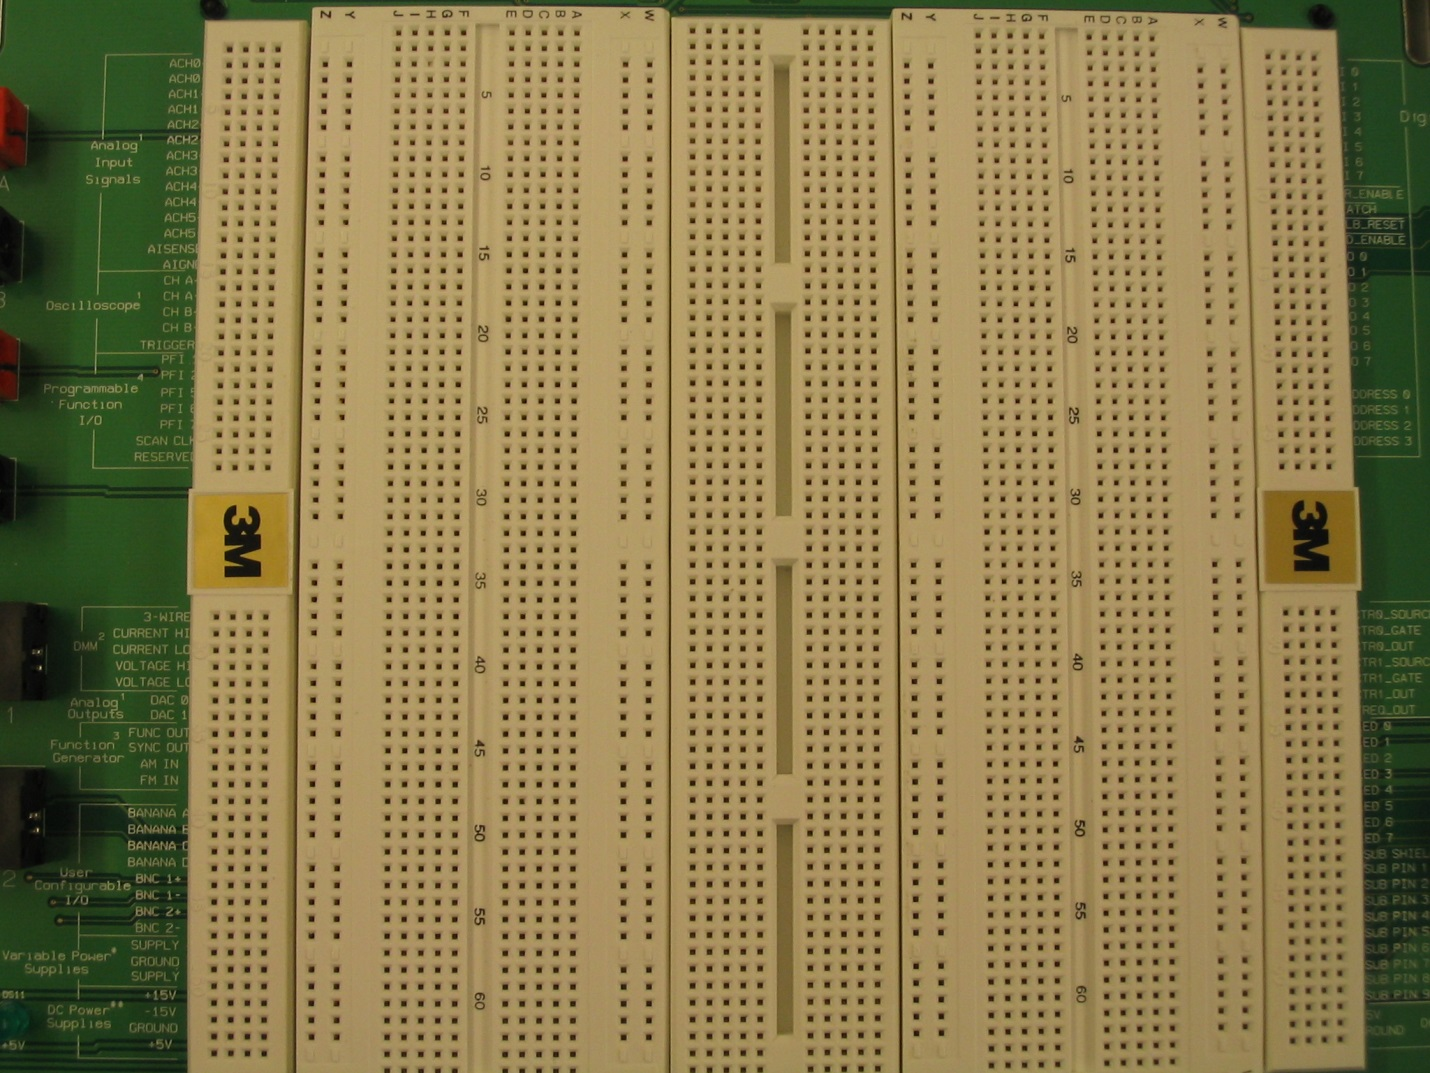
\includegraphics[width=\textwidth]{lab_1_fig_9.jpg}
    	\centering
		\end{figure}\\TA check: \underline{\hspace{2cm}}
\end{itemize}
\pagebreak

\section*{Part 2: DC Analysis of Simple Circuits}

\subsection*{Voltage Divider}
\begin{itemize}
	\item What is the relationship between the input voltage, V\_in, and the output voltage, V\_out, in terms of R1 and R2?\vspace{3cm}
	\item Assume that we want H = 0.5 for the voltage divider. If R2 = 100 \textOmega, what should R1 be?\vspace{2cm}
	\item Construct a voltage divider on the ELVIS protoboard using the values of R1 and R2 from part 3 above. Do not apply V\_IN yet.\\TA check: \underline{\hspace{2cm}}
	\item What output do you expect? What output do you see? \textit{If your output doesn’t quite match what you expected to see, why do you think this is the case? If your output does match what you expect, can you speculate why it wouldn’t? Where are inaccuracies most likely to come from?}\vspace{4cm}
	\item Rearrange your voltage divider to obtain a transfer function H= 0.3. Input a sinusoidal signal into your voltage divider. Show the TA your results. Describe the results you obtain.\\TA check: \underline{\hspace{2cm}}
\end{itemize}
\pagebreak

\subsection*{Variable Resistor}
\begin{itemize}
	\item Using an external DMM to adjust the resistance across the two connected terminals of your potentiometer, and the ELVIS oscilloscope to measure the voltage across your potentiometer, calculate current output across your ‘load’.

		\begin{table}[h!]
		\centering
		\begin{tabular}[h!]{c|c|c}
		\toprule
		Resistance (\textOmega) & Voltage across the pot (V) & Current (I) \\
		\midrule
		10 & &\\
		\midrule
		50 & &\\
		\midrule
		100 & &\\
		\midrule
		150 & &\\
		\midrule
		200 & &\\
		\bottomrule
		\end{tabular}
		\end{table}
		
	\item What would happen if the resistance between your connected terminals is decreased until it reads 0\textOmega?\vspace{2cm}
	\item Explain how this is circuit is working and possible applications of this setup. \textit{Hint: if you are still not sure about what you are seeing, connect an external DMM to measure the current as you adjust your pot.}\\TA check: \underline{\hspace{2cm}}
\end{itemize}

\subsection*{Voltage Divider}
\begin{itemize}
	\item Using the virtual NI ELVIS II oscilloscope, describe the behavior you observe in Ch0, Ch1 and Ch2 as you turn the knob on the potentiometer.\vspace{2cm}
	\item Explain how this is circuit is working and possible applications of this setup.\\TA check: \underline{\hspace{2cm}}\vspace{2cm}
\end{itemize}

\subsection*{Wheatstone Bridge}
\begin{itemize}
	\item Using the values of R1 and R2 from part (I), what do you expect the value of V\_a to be in terms of V\_in? What about V\_b?\vspace{2cm}
	\item If you consider your output, “V\_out”, to be the difference between V\_a and V\_b, what would you expect this output to be?\vspace{2cm}
	\item Construct the Wheatstone bridge by building off of your circuit from part (I).\\TA check: \underline{\hspace{2cm}}
	\item Apply a DC voltage across the V\_in terminals (you can use the same input from part (I)), and measure the potential at V\_a. Measure V\_b. Are they the same? If not, why not?\vspace{2cm}
	\item With no strain applied to the gage, we require V\_a = V\_b, which would result in V\_out = 0. i.e. a balanced bridge. This is necessary to be able to accurately detect changes in strain when resistance changes in any one arm of the bridge. To do this, we can substitute a potentiometer and balance the bridge. Replace R2 with a 200 \textOmega pot (use rheostat configuration from above). Balance the bridge by measuring V\_out and adjust the pot resistance until V\_out = 0.
	\item Now that you have balanced the bridge, gently bend the material. You don’t want to create a permanent deformation or break it – so please be gentle. What do you see? How does the circuit output vary in response to compression and tension? Qualitatively, how sensitive is the strain gauge?\vspace{3cm}
	\item How does the relative change in resistance of the gage depend on the applied strain? How would the output voltage of the bridge relate to the strain? Why does it make sense to have the baseline V\_out = 0?\\TA check: \underline{\hspace{2cm}}
\end{itemize}
\end{document}
